\documentclass[11pt]{article}
\pdfinfoomitdate=1
\pdftrailerid{}
\pdfsuppressptexinfo=15
\usepackage[T1]{fontenc}
\usepackage[utf8]{inputenc}
\usepackage{lmodern}
\usepackage[margin=1in]{geometry}
\usepackage{amsmath,amssymb,amsthm,mathtools}
\usepackage{microtype,tikz,xcolor}
\usetikzlibrary{arrows.meta,patterns,calc}
\usepackage[unicode,colorlinks=true,linkcolor=blue!45!black,citecolor=blue!45!black,urlcolor=blue!45!black]{hyperref}
\urlstyle{same}
\expandafter\def\expandafter\UrlBreaks\expandafter{\UrlBreaks\do\-}
\hypersetup{pdftitle={Ultraflat real Littlewood polynomials},pdfauthor={OpenAI}}
\newcommand{\T}{\mathbb T}
\newcommand{\R}{\mathbb R}
\newcommand{\Z}{\mathbb Z}
\newcommand{\N}{\mathbb N}
\newcommand{\C}{\mathbb C}
\newcommand{\e}{\mathrm e}
\newcommand{\norm}[1]{\lVert #1\rVert}
\DeclareMathOperator{\sgn}{sgn}
\DeclareMathOperator{\supp}{supp}
\newtheorem{theorem}{Theorem}
\newtheorem{lemma}{Lemma}[section]
\newtheorem{proposition}[lemma]{Proposition}
\newtheorem{corollary}[lemma]{Corollary}
\theoremstyle{remark}
\newtheorem{remark}[lemma]{Remark}
\numberwithin{equation}{section}
\setlength{\emergencystretch}{2em}
\allowdisplaybreaks[2]
\title{Ultraflat real Littlewood polynomials}
\author{OpenAI}
\date{October 5, 2026}
\begin{document}
\maketitle
\begin{abstract}
For every $\varepsilon\in(0,1)$ and every sufficiently large integer $N$,
there is a polynomial of length $N$ with coefficients in $\{-1,1\}$ whose
modulus lies between $(1-\varepsilon)\sqrt N$ and
$(1+\varepsilon)\sqrt N$ everywhere on the unit circle. Thus real
Littlewood polynomials can be ultraflat through every sufficiently large
integer length. The signs may be chosen separately at each length.
\end{abstract}
\section{Introduction}\label{sec:introduction}

A real Littlewood polynomial of length $N$ is a polynomial
\[
 P(z)=\sum_{k=0}^{N-1}\varepsilon_k z^k,
 \qquad \varepsilon_k\in\{-1,1\}.
\]
Its squared mean modulus on the unit circle is $N$, by Parseval's
identity. Thus $\sqrt N$ is the natural scale, and its maximum modulus
is at least $\sqrt N$. A family is \emph{ultraflat} if
$|P(z)|/\sqrt N$ tends uniformly to $1$ on the unit circle as the
length tends to infinity. We prove that real Littlewood polynomials
can be ultraflat, through every sufficiently large integer length.

\begin{theorem}\label{thm:main}
For every $\varepsilon\in(0,1)$ there is an integer $N_0$ such that,
for every integer $N\ge N_0$, there are signs
$\varepsilon_0,\ldots,\varepsilon_{N-1}$ for which
\[
 (1-\varepsilon)\sqrt N
 \le\left|\sum_{k=0}^{N-1}\varepsilon_k z^k\right|
 \le(1+\varepsilon)\sqrt N
 \qquad\text{for every }|z|=1.
\]
\end{theorem}

The signs may depend on $N$. The theorem concerns both extrema of the
same polynomial on the entire circle, including the real points
$z=1$ and $z=-1$.

\subsection{The flatness problem}

Erd\H{o}s asked whether real-sign polynomials could stay between two
fixed positive multiples of their square-root scale on the entire
circle \cite[Problem~26]{Erdos1957}; the problem also appears in
Littlewood's work \cite{Littlewood1966}. The Rudin--Shapiro construction
gives real-sign polynomials with maximum at most $\sqrt{2N}$ at dyadic
lengths \cite{Rudin1959}. Balister, Bollob\'as, Morris, Sahasrabudhe and
Tiba proved the two-sided constant-factor statement at every degree
at least two \cite[Theorem~1.1]{BalisterEtAl2020}. Their theorem controls
the scale of both extrema, while ultraflatness requires both normalized
extrema to converge to one.

For complex coefficients of modulus one, Kahane constructed ultraflat
polynomials \cite{Kahane1980}. Bombieri and Bourgain improved the
quantitative bounds and gave effective constructions
\cite[Theorems~4 and~7]{BombieriBourgain2009}. The restriction to real
signs is substantial. The predecessor \cite[Theorem~1.1]{OpenAIMinimal}
obtains an asymptotically minimal maximum through all lengths. Its
version-2 refinement \cite[Theorem~1.1]{OpenAILowerEnvelope2026} gives
the simultaneous bounds
\[
 \frac1{16}\sqrt N\le |P(z)|\le(1+\eta)\sqrt N
 \qquad(|z|=1)
\]
for every fixed $\eta>0$ and all sufficiently large $N$.
Theorem~\ref{thm:main} strengthens that lower bound to its asymptotically
optimal value. The present paper develops the additional constructions
needed for this strengthening and uses the retained version-2 paper
as the source of two shared lemmas.

Recent obstructions distinguish the relevant quantifiers. Erd\'elyi
proved that the full sequence of partial sums of one fixed unimodular
power series cannot be ultraflat
\cite[Theorem~2.1]{ErdelyiSections2026}. This does not restrict the
independent choice of signs at each length in Theorem~\ref{thm:main}.
His separate lower bound
\cite[Theorem~2.1]{Erdelyi2026},
$\max_{|z|=1}|P(z)|^2\ge N+(N-1)^{1/3}/38$, is compatible with
the asymptotic conclusion here.\footnote{Contrary nonflatness claims
in \cite{ElAbdalaoui2025,ElAbdalaoui2025Generalization} and specific
issues in their arguments are discussed in
\cite[Appendix~A]{OpenAIMinimal}. Those claims are not inputs to the
present proof.}

\subsection{Construction and relation to the earlier version}

The proof first constructs a continuous function $B_N$ on the circle
whose modulus is close to one. Its Fourier coefficients of indices
$0,\ldots,N-1$ are real and at most $(1+o(1))/\sqrt N$ in absolute
value, and the sum of the absolute values of all remaining coefficients
tends to zero. Parseval's identity then forces the retained coefficients
to be almost of sign size in aggregate. A discrepancy estimate rounds
them to signs with a small uniform error. This last passage converts
the continuous construction into a Littlewood polynomial.

To build $B_N$, we adapt the auxiliary-torus and phase-correction
arguments of \cite[Sections~2, 4, and~5]{OpenAILowerEnvelope2026}.
The auxiliary object is a real trigonometric polynomial
$F(y)=\sum_{a\in\mathcal A}c_a\e(a\cdot y)$ on a higher-dimensional
torus, where $\e(t)=\exp(2\pi i t)$. Its norm is at most $1+\delta$,
and its Fourier coefficients
are compared with positive weights $w_a=|a\cdot v|$ whose sum is
close to one. Here $\delta>0$ is a small error parameter and $v$ is
a fixed real vector. The first additional requirement is the two-sided
comparison
\[
 1\le |c_a|/\sqrt{w_a}\le1+C\delta.
\]
We obtain it by spreading each original coefficient over a box of
frequencies and rounding the spreading factors to equal coefficient
magnitudes. Section~\ref{sec:rounding} proves the required complex
version of the defect-sensitive rounding estimate, and
Section~\ref{sec:balanced} carries out the auxiliary construction.

The frequencies of $F$ then supply oscillatory waves on disjoint short
arcs, each with constant modulus $|c_a|/\sqrt{w_a}$. Their phases are
chosen so that, at a fixed Fourier index, the leading stationary-phase
terms sum to a single value of $F$ multiplied by a factor in $[0,1]$.
The norm bound for $F$ therefore controls these contributions without accumulating
the magnitudes of its coefficients.

The second change concerns the endpoints of the waves. We increase the
magnitude of their phase curvature near the endpoints while keeping
their amplitudes constant. Stationary phase
therefore gives small endpoint Fourier contributions while the
function's modulus stays close to one. The waves are joined across
the remaining gaps by matching their values and their leading phase
derivatives. These matching conditions cancel the first boundary terms
in integration by parts and give a summable exterior Fourier tail.
Section~\ref{sec:oscillation} supplies the analytic estimates,
Section~\ref{sec:waves} constructs and joins the waves, and
Section~\ref{sec:completion} projects and rounds to signs.

The signed interval packing and real matrix discrepancy lemmas are
inherited from \cite[Lemmas~3.1 and~6.2]{OpenAILowerEnvelope2026}.
Their combinatorial inputs are the Pippenger--Spencer hypergraph-coloring
theorem \cite{PippengerSpencer1989}, in the quantified form of
\cite[Lemma~2.1]{AlonYuster2005}, and the partial-coloring method of
Spencer \cite{Spencer1985} and Lovett--Meka \cite{LovettMeka2015}.
Discrepancy and the repair of exceptional arcs also occur in
\cite[Sections~2.1 and~4]{BalisterEtAl2020}, where a sine polynomial
corrects a Rudin--Shapiro cosine polynomial. Here the correction joins
oscillatory waves while preserving their almost constant modulus.
All dimensions, packing data, intervals, and leading phases are fixed before
the final length tends to infinity; the construction consequently
applies to all sufficiently large integer lengths.

\section{Oscillatory integral estimates}\label{sec:oscillation}

Throughout, $\T=\R/\Z$, $\e(t)=\exp(2\pi i t)$, and Haar measure on
each torus has mass one. We use the Fourier convention
$\widehat f(k)=\int_\T f(t)\e(-kt)\,dt$, and the same convention on
$\R$. Constants denoted by $C$ are absolute and may change from line
to line. Subscripts indicate dependence on fixed data. The length
$N$ will tend to infinity only after all auxiliary data have been fixed.

We record three elementary forms of stationary phase. The first supplies
uniform control of every coefficient of a truncated quadratic wave.
The second identifies the leading coefficients of the main construction;
the third handles its small end pieces and gaps.

\begin{lemma}[Uniform quadratic formula]\label{lem:quadratic}
Let $g\in C_c^\infty(\R)$ and $\beta\in\R\setminus\{0\}$. As
$T\to\infty$, uniformly for all $u\in\R$,
\begin{equation}\label{eq:quadratic-formula}
 \int_\R g(y)\e(T\beta y^2/2-uy)\,dy
 =\frac{\e(\sgn(\beta)/8-u^2/(2T\beta))}{\sqrt{T|\beta|}}
   \left[g\left(\frac{u}{T\beta}\right)+O_{g,\beta}(T^{-1})\right].
\end{equation}
\end{lemma}
\begin{proof}
Put $y_0=u/(T\beta)$ and complete the square. Fourier inversion reduces
the bracket in \eqref{eq:quadratic-formula} to the exact expression
\[
 \int_\R \widehat g(\xi)\e(\xi y_0)
                     \e\bigl(-\xi^2/(2T\beta)\bigr)\,d\xi.
\]
For completeness, this identity follows by inserting
$\exp(-\pi r(y-y_0)^2)$, $r>0$, before applying Fourier inversion.
The inner Gaussian integral has factor
$(r-iT\beta)^{-1/2}\exp(-\pi\xi^2/(r-iT\beta))$;
its modulus is at most $(T|\beta|)^{-1/2}$. Dominated convergence
against $|\widehat g(\xi)|$ justifies $r\downarrow0$ and yields the
factor $\e(\sgn(\beta)/8)/\sqrt{T|\beta|}$.
Finally, replacing $\e(-\xi^2/(2T\beta))$ by $1$ costs at most
\[
 \frac{\pi}{T|\beta|}\int_\R \xi^2|\widehat g(\xi)|\,d\xi,
\]
independently of $y_0$.
\end{proof}

\begin{lemma}[Uniform stationary phase]\label{lem:stationary-phase}
Let $I$ be a compact interval, let $\phi$ be smooth on a neighborhood
of $I$ with $\phi''$ nowhere zero there, and let
$f\in C_c^\infty(\operatorname{int}I)$. Uniformly for $x\in[0,1]$,
\begin{equation}\label{eq:stationary-phase}
 \sqrt N\int_I f(t)\e\bigl(N(\phi(t)-xt)\bigr)\,dt
 =\frac{f(t_x)}{\sqrt{|\phi''(t_x)|}}
   \e\bigl(N(\phi(t_x)-xt_x)+\sgn(\phi'')/8\bigr)+o(1),
\end{equation}
where $t_x$ is the unique point with $\phi'(t_x)=x$ if it exists in
$I$, and the right-hand main term is zero otherwise.
\end{lemma}
\begin{proof}
Write $d=\sgn(\phi'')$. If $t_x\in I$, the change of variable
\[
 y=(t-t_x)
 \left(\frac{2d[\phi(t)-\phi(t_x)-\phi'(t_x)(t-t_x)]}
 {(t-t_x)^2}\right)^{1/2}
\]
extends smoothly across $t=t_x$ and changes the phase to
$\phi(t_x)-xt_x+dy^2/2$. Taylor's integral formula and the lower
bound on $|\phi''|$ show that this is a smooth increasing coordinate
with derivative bounded above and below, uniformly for $t_x\in I$.
All its required derivatives and those of its inverse are uniformly
bounded. The transformed amplitudes, extended by zero, have support
in a fixed compact set and uniformly bounded smooth norms, because
$\supp f$ is separated from the endpoints of $I$. At $y=0$ their
value is $f(t_x)/\sqrt{|\phi''(t_x)|}$.
Lemma~\ref{lem:quadratic}, whose error is controlled by a fixed finite
collection of smooth norms, proves the assertion uniformly in this
case. If $x\notin\phi'(I)$, the distance between $x$ and
$\phi'(\supp f)$ is bounded below uniformly; integration by parts
then gives an $O(N^{-1})$ integral. These two cases include the
endpoints of $\phi'(I)$.
\end{proof}

\begin{lemma}[Bounds with endpoint amplitudes]\label{lem:oscillatory-bounds}
Let $I$ be a compact interval, $f\in C^1(I)$, and $\phi$ be real and smooth.
If $\phi''=\Lambda\ne0$ on $I$, then for all real $k$,
\begin{equation}\label{eq:quadratic-bound}
 \left|\int_I f(t)\e(N\phi(t)-kt)\,dt\right|
 \le\frac{C}{\sqrt{N|\Lambda|}}
       \left(\norm f_\infty+\int_I|f'(t)|\,dt\right).
\end{equation}
If $N\phi'-k$ is monotone and has absolute value at least $N\rho>0$,
the same bound holds with $C/(N\rho)$ in place of
$C/\sqrt{N|\Lambda|}$.
\end{lemma}
\begin{proof}
The primitive of $\e(\pm y^2/2)$ has bounded differences on arbitrary
real intervals: inside $[-1,1]$ this is immediate, and on either
remaining half-line integration by parts gives a uniform bound.
Completing the square and rescaling therefore bounds every subinterval
integral of $\e(N\phi-kt)$ by $C/\sqrt{N|\Lambda|}$ in the quadratic
case. In the monotone case, one integration by parts bounds every such
integral by $C/(N\rho)$; monotonicity bounds the total variation of
$(N\phi'-k)^{-1}$ by $2/(N\rho)$. Integration against the amplitude
$f$, using either primitive, gives the stated estimates.
\end{proof}

\section{Rounding with a small defect}\label{sec:rounding}

We need to round almost unimodular coefficients while controlling the
error on the whole circle.  The estimate below extends the real rounding
argument of \cite[Section~6]{OpenAILowerEnvelope2026} to prescribed complex
phases.  We quote its real matrix discrepancy lemma below; the proof
there uses the partial-coloring method of Spencer \cite{Spencer1985}
and the real-vector theorem of Lovett and Meka
\cite[Theorem~4 of arXiv:1203.5747v2]{LovettMeka2015}.

\begin{lemma}[Real matrix discrepancy]\label{lem:matrix-discrepancy}
There is an absolute constant $C$ such that, for integers $1\le s\le R$
and every $A\in[-1,1]^{R\times s}$, there is a vector
$\xi\in\{-1,1\}^s$ satisfying
\[
 \norm{A\xi}_\infty\le C\sqrt{s\log(2R/s)}.
\]
\end{lemma}

\begin{proof}
This is \cite[Lemma~6.2]{OpenAILowerEnvelope2026}, whose statement applies
to arbitrary real matrices in the displayed rectangular range.
\end{proof}

\begin{lemma}[Rounding with prescribed phases]\label{lem:complex-rounding}
Let $n\ge1$ be an integer and $Z_0,\ldots,Z_{n-1}\in\C$ satisfy
$|Z_j|\le1$.  Write $Z_j=d_j|Z_j|$, where $|d_j|=1$, choosing $d_j=1$
when $Z_j=0$, and put
\[
 \mu=\frac12\sum_{j=0}^{n-1}(1-|Z_j|).
\]
There are $\eta_j\in\{d_j,-d_j\}$ such that
\begin{equation}\label{eq:complex-rounding}
 \sup_{t\in\T}\left|\sum_{j=0}^{n-1}(\eta_j-Z_j)\e(jt)\right|
 \le C\left(1+\sqrt{\mu\log(80n/\mu)}\right),
\end{equation}
with an absolute constant $C$.  The square-root term is zero for
$\mu=0$, when the error can be zero.  For real inputs the outputs are
real signs.  The same estimate holds on any interval of $n$ consecutive
integer frequencies.
\end{lemma}

\begin{proof}
If $\mu=0$, take $\eta_j=Z_j$.  Suppose $\mu>0$, and set
$p_j=(1-|Z_j|)/2$.  Then $0\le p_j\le1/2$ and $\sum_jp_j=\mu$.
On the grid $t_\ell=\ell/(20n)$, $0\le\ell<20n$, form the real matrix
with $R=40n$ rows
\[
 A_{2\ell,j}=\Re\bigl(d_j\e(jt_\ell)\bigr),\qquad
 A_{2\ell+1,j}=\Im\bigl(d_j\e(jt_\ell)\bigr).
\]
Every entry belongs to $[-1,1]$.  We round $p$ to a vector in
$\{0,1\}^n$, preserving an upper bound on its total mass.

Choose an integer $J\ge1$ with $n2^{-J}\le1$, and first set
$p_j^{(J)}=2^{-J}\lfloor2^Jp_j\rfloor$.  This costs at most $1$ in
$\norm{A(p^{(J)}-p)}_\infty$ and does not increase the mass.
At stage $h=J,\ldots,1$, let $S_h$ contain those coordinates for which
$2^hp_j^{(h)}$ is odd, and let $s_h=|S_h|$.  If $s_h=0$, leave the
vector unchanged.  Otherwise apply Lemma~\ref{lem:matrix-discrepancy}
to the columns indexed by $S_h$.  Reverse all its signs if necessary so
that their sum is nonpositive, and put
\[
 p_j^{(h-1)}=
 \begin{cases}
 p_j^{(h)}+2^{-h}\xi_j,&j\in S_h,\\
 p_j^{(h)},&j\notin S_h.
 \end{cases}
\]
An odd multiple of $2^{-h}$ in $[0,1]$ lies between $2^{-h}$ and
$1-2^{-h}$.  Either change therefore stays in $[0,1]$ and lies on the
next coarser grid.  The total mass remains at most $\mu$, while the
simultaneous sign reversal leaves the absolute discrepancy unchanged.
In particular, each active coordinate has mass at least $2^{-h}$, so
\[
 s_h\le\min(n,2^h\mu),\qquad
 \norm{A(p^{(h-1)}-p^{(h)})}_\infty
 \le C2^{-h}\sqrt{s_h\log(80n/s_h)}.
\]
The last inequality is used only at nonempty stages.  Monotonicity of
$s\log(80n/s)$ on $(0,n]$ gives
\[
 s_h\log(80n/s_h)\le2^h\mu\log(80n/\mu).
\]
For $2^h\mu>n$, use the bound $n\log80$ on the left and
$\mu\le n/2$ on the right.  Summing the geometric series of step errors
yields, with $p'=p^{(0)}\in\{0,1\}^n$,
\begin{equation}\label{eq:rounding-matrix-error}
 \norm{A(p'-p)}_\infty
 \le1+C\sqrt{\mu\log(80n/\mu)}.
\end{equation}

Set $\eta_j=d_j(1-2p'_j)$ and
$Q(z)=\sum_{j=0}^{n-1}(\eta_j-Z_j)z^j$.
The real and imaginary parts of $Q(\e(t_\ell))$ are each bounded by
twice the left side of \eqref{eq:rounding-matrix-error}.  Thus the
claimed error bound holds on the grid.
To pass to the circle, let $S=\max_{|z|=1}|Q(z)|$.  The maximum principle,
applied also to the reversed polynomial, gives
\[
 |Q(z)|\le S\max(1,|z|^{n-1}),\qquad
 \max_{|z|\le1+1/n}|Q(z)|\le\exp(1)S.
\]
Cauchy's estimate in disks of radius $1/n$ centered on the unit circle
therefore gives
\[
 \left|\frac{d}{dt}Q(\e(t))\right|\le2\pi\exp(1)nS.
\]
Every point of $\T$ is within $1/(40n)$ of the grid.  Hence
$S\le\max_\ell|Q(\e(t_\ell))|+(\pi\exp(1)/20)S$.
Since $\pi\exp(1)/20<1$, this proves
\eqref{eq:complex-rounding}.  Multiplication by a unimodular monomial
handles shifted consecutive frequencies.  If the inputs are real,
all $d_j$ are signs and hence so are the outputs.
\end{proof}

\section{A real auxiliary function with balanced coefficients}\label{sec:balanced}

The wave construction will use a bounded real trigonometric polynomial
whose coefficient magnitudes are close to the square roots of its
frequency weights.  These weights must have the form $|a\cdot v|$, where
$a$ is a Fourier frequency and $v$ is one common vector.  We adapt the auxiliary-torus construction of
\cite[Section~2]{OpenAILowerEnvelope2026}.  The additional step is to
round the coefficients of each spreading factor to a common magnitude.

\begin{proposition}\label{prop:balanced}
For every $0<\delta<1/100$, there are an integer $m\ge2$, a real
trigonometric polynomial $F$ on $\T^m$, and $v\in\R^m$ with the
following properties.  Its Fourier support
$\mathcal A\subset\Z^m\setminus\{0\}$ consists of at least two pairs
$\{a,-a\}$, with distinct pairs nonparallel.  If
\[
 c_a=\widehat F(a),\qquad \lambda_a=a\cdot v,\qquad w_a=|\lambda_a|,
\]
then, for an absolute constant $C$,
\begin{equation}\label{eq:balanced}
 \begin{gathered}
 \norm F_\infty\le1+\delta,\qquad w_a>0,\\
 1-C\delta\le\sum_{a\in\mathcal A}w_a<1,\qquad
 1\le\frac{|c_a|}{\sqrt{w_a}}\le1+C\delta
 \quad(a\in\mathcal A).
 \end{gathered}
\end{equation}
The coefficient ratios in \eqref{eq:balanced} are also at most $2$.
\end{proposition}

We first construct the one-dimensional factors that will spread each
original frequency into a box.  The requirement that every coefficient
have the same magnitude makes the later comparison with $w_a$ exact.

\begin{lemma}[Spreading with equal coefficient magnitudes]
\label{lem:equal-modulus-spreading}
Let $\mathcal B\subset\R\setminus\{0\}$ be finite and invariant under
negation.  For every $\alpha>0$, there is a real
$g\in C_c^\infty((-1/2,1/2))$, with $0\le g\le1$, such that for every
sufficiently large real $T$ and each $\beta\in\mathcal B$ there is a
trigonometric polynomial
\[
 f_\beta(y)=\sum_{|u|\le\lfloor T|\beta|/2\rfloor}a_{\beta,u}\e(uy),
 \qquad
 |a_{\beta,u}|=L_\beta^{-1/2},\qquad
 L_\beta=2\lfloor T|\beta|/2\rfloor+1,
\]
satisfying
\begin{equation}\label{eq:spreading-approximation}
 \norm{f_\beta-g(\,\cdot\,)\e(T\beta(\,\cdot\,)^2/2)}_\infty\le\alpha.
\end{equation}
Here the target is extended periodically from $[-1/2,1/2]$, and the
choices may satisfy $f_{-\beta}=\overline{f_\beta}$.
\end{lemma}

\begin{proof}
Choose $0<q<1/4$, to be fixed in terms of $\alpha$, and then
choose such a $g$ with $\int g^2\ge1-q$.
For a fixed $\beta\in\mathcal B$, write
\[
 I_\beta(u)=\int_{-1/2}^{1/2}g(y)\e(T\beta y^2/2-uy)\,dy
 \qquad(u\in\Z).
\]
Lemma~\ref{lem:quadratic} and $L_\beta/(T|\beta|)\to1$ give, uniformly
in $u$,
\begin{equation}\label{eq:spreading-coefficient-bound}
 \sqrt{L_\beta}|I_\beta(u)|\le1+q
\end{equation}
for all sufficiently large $T$.
The coefficients outside the stated interval have a small sum of
absolute values.  Indeed, $\supp g$ is separated from both endpoints,
so on a neighborhood of this support,
\[
 |T\beta y-u|\ge c_{g,\beta}(T+|u|)
 \quad\text{if }|u|>T|\beta|/2.
\]
Twice integrating by parts, with no boundary terms, gives
$|I_\beta(u)|\le C_{g,\beta}(T+|u|)^{-2}$ there.  The derivative of
$T\beta y-u$ is $T\beta$, so all terms from these integrations have
this bound.  Consequently
\begin{equation}\label{eq:spreading-tail}
 \sum_{|u|>\lfloor T|\beta|/2\rfloor}|I_\beta(u)|=O_{g,\beta}(T^{-1}).
\end{equation}

For the retained indices define
$Z_u=\sqrt{L_\beta}I_\beta(u)/(1+q)$.
By \eqref{eq:spreading-coefficient-bound}, $|Z_u|\le1$.
Parseval's identity and \eqref{eq:spreading-tail} show that, for large $T$,
\[
 \frac1{L_\beta}\sum_u|Z_u|^2\ge\frac{1-2q}{(1+q)^2}.
\]
Since $1-|Z_u|\le1-|Z_u|^2$, the defect
$\mu=\frac12\sum_u(1-|Z_u|)$ satisfies
\[
 \frac{\mu}{L_\beta}\le\frac{4q+q^2}{2(1+q)^2}\le2q<1/2.
\]
Apply Lemma~\ref{lem:complex-rounding} on this consecutive interval of
frequencies, and divide its conclusion by $\sqrt{L_\beta}$.  It gives
unit complex numbers $\eta_u$.  Their polynomial
$f_\beta(y)=\sum_u L_\beta^{-1/2}\eta_u\e(uy)$ satisfies
\[
 \norm{f_\beta-\frac1{1+q}\sum_u I_\beta(u)\e(u\,\cdot)}_\infty
 \le C\left(L_\beta^{-1/2}+\sqrt{q\log(80/q)}\right).
\]
Indeed, for $x=\mu/L_\beta>0$, monotonicity gives
$x\log(80/x)\le2q\log(40/q)\le2q\log(80/q)$; the zero-defect
case follows directly from the rounding lemma.  By \eqref{eq:spreading-tail}, the polynomial before rounding
differs from the target by at most $q+o(1)$ in supremum norm.
First choose $q$ small enough, then fix $g$, and finally take $T$ large.
The resulting error is at most $\alpha$.
All estimates hold simultaneously for the finite set $\mathcal B$.
Construct the polynomials for positive $\beta$ and set
$f_{-\beta}=\overline{f_\beta}$: the targets are conjugates and the
frequency intervals are symmetric, so all conclusions are preserved.
\end{proof}

\begin{proof}[Proof of Proposition~\ref{prop:balanced}]
We first construct a real polynomial with norm at most one and squared
$L^2$ norm close to one.  Starting with $p_0=0$, define successively
\[
 p_j(y_1,\ldots,y_j)
 =p_{j-1}(y_1,\ldots,y_{j-1})
  +\tfrac12(1-p_{j-1}(y_1,\ldots,y_{j-1})^2)\cos(2\pi y_j).
\]
These polynomials have mean zero and satisfy $|p_j|\le1$, because
$(1-r^2)/2\le1-|r|$ for $|r|\le1$.
Writing $M_j=\int p_j^2$, integration in the new coordinate gives
\[
 M_j-M_{j-1}=\tfrac18\int(1-p_{j-1}^2)^2
 \ge\tfrac18(1-M_{j-1})^2.
\]
Thus $M_j\uparrow1$: a limit smaller than one would force increments
bounded away from zero.  Fix $d\ge2$ with $M_d\ge1-\delta$, and write
\[
 p_d(y)=\sum_{s\in\mathcal S}b_s\e(s\cdot y),
 \qquad b_s\ne0.
\]
Zero is not in $\mathcal S$, since $p_d$ has mean zero.  At each step,
old frequencies acquire a zero final coordinate and persist, while
new frequencies have final coordinate $1$ or $-1$.  Hence every
$s\in\mathcal S$ has last nonzero coordinate $1$ or $-1$.
Parallel members of $\mathcal S$ are therefore equal up to sign.
The first-coordinate pair persists, and the second step introduces
another pair, since $\int(1-p_1^2)>0$.
Choose representatives $s_1,\ldots,s_D$ of these sign pairs.

We next choose the sizes of the frequency boxes.  Choose
$\gamma\in\R^d$ outside the finitely many hyperplanes $s^\perp$, and
put $\rho_s=|s\cdot\gamma|>0$.  The box over $s$ should contain a
number of frequencies approximately proportional to $|b_s|^2/\rho_s$:
equal spreading then makes each squared coefficient approximately
proportional to $\rho_s$, matching the weight supplied by a vector $v$
proportional to $(\gamma,0)$.  We will choose vectors
$W_1,\ldots,W_D\in\R^d$ with nonzero projections $s\cdot W_j$ and use
these projections as spreading parameters.  The box over $s$ will then
have size asymptotic to $T^D\prod_j|s\cdot W_j|$.  We therefore require
these products to be approximately $\tau|b_s|^2/\rho_s$, using one
small positive parameter $\tau$ for all $s$.

For each $j$, choose $W_j^0\in s_j^\perp$ not orthogonal to any other
representative.  This is possible because $d\ge2$ and the representatives
are pairwise nonparallel, so only finitely many proper subspaces of
$s_j^\perp$ are excluded.  Choose $W_j^1\in\R^d$ such that
\[
 s_j\cdot W_j^1
 =\frac{|b_{s_j}|^2}
 {\rho_{s_j}\prod_{\ell\ne j}|s_j\cdot W_\ell^0|}.
\]
Set $W_j=W_j^0+\tau W_j^1$.  As $\tau\downarrow0$,
\[
 \frac1\tau\prod_{j=1}^D|s\cdot W_j|
 \longrightarrow\frac{|b_s|^2}{\rho_s}
 \qquad(s\in\mathcal S).
\]
Indeed, exactly the factor belonging to the representative of $\{s,-s\}$
vanishes at $\tau=0$, and its first-order coefficient was just prescribed.
Fix $\tau>0$ small enough that all factors are nonzero and, with
$\beta_{s,j}=s\cdot W_j$ and $\Delta_s=\prod_j|\beta_{s,j}|$,
\begin{equation}\label{eq:projection-products}
 (1-\delta)\frac{\tau|b_s|^2}{\rho_s}
 \le\Delta_s\le
 (1+\delta)\frac{\tau|b_s|^2}{\rho_s}
 \qquad(s\in\mathcal S).
\end{equation}

All these data are now fixed.  Apply
Lemma~\ref{lem:equal-modulus-spreading} to the finite list of nonzero
$\beta_{s,j}$, choosing $\alpha>0$ small enough that
\begin{equation}\label{eq:balanced-product-error}
 \left(\sum_{s\in\mathcal S}|b_s|\right)
 D\alpha(1+\alpha)^{D-1}\le\delta.
\end{equation}
With the resulting common cutoff $g$ and sufficiently large $T$, define
\[
 F(y,z)=\sum_{s\in\mathcal S}b_s\e(s\cdot y)
                  \prod_{j=1}^D f_{\beta_{s,j}}(z_j),
 \qquad (y,z)\in\T^d\times\T^D.
\]
The conjugation condition on the factors and
$b_{-s}=\overline{b_s}$ show that $F$ is real.
If each factor is replaced by its target, the resulting function is
\[
 \left(\prod_{j=1}^Dg(z_j)\right)
 p_d\left(y+\frac T2\sum_{j=1}^D W_jz_j^2\right),
\]
where $z_j$ is represented in $[-1/2,1/2]$.  The cutoffs vanish near
the endpoints, so this expression is well defined on the torus and has
norm at most one.  A telescoping product estimate bounds its distance
from $F$ by the left side of \eqref{eq:balanced-product-error}.
Therefore $\norm F_\infty\le1+\delta$.

Over each old frequency $s$, the Fourier support of $F$ is the full box
\[
 a=(s,u_1,\ldots,u_D),\qquad
 |u_j|\le\lfloor T|\beta_{s,j}|/2\rfloor.
\]
This box has $n_s=\prod_jL_{\beta_{s,j}}$ members, each with coefficient
magnitude $|b_s|/\sqrt{n_s}$.  Distinct old frequencies give disjoint
boxes, so every indicated coefficient is nonzero.  If two resulting
frequencies are parallel, their $s$ coordinates force the proportionality
factor to be $1$ or $-1$; thus they are equal or opposite.  There remain
at least two sign pairs, and no zero frequency.

Since $L_\beta/(T|\beta|)\to1$, increase $T$ so that
\begin{equation}\label{eq:box-sizes}
 (1-\delta)T^D\Delta_s\le n_s\le(1+\delta)T^D\Delta_s
 \qquad(s\in\mathcal S),
\end{equation}
and choose the approximants at this value of $T$.  This is permitted
because the spreading lemma holds for every sufficiently large $T$.
Fix $T$, put $m=d+D$, and take
\[
 v=\left(\frac{\gamma}{\tau T^D(1+\delta)^3},0\right)\in\R^{d+D}.
\]
For every frequency $a$ over $s$, its weight is
$w_a=\rho_s/(\tau T^D(1+\delta)^3)>0$.
Combining \eqref{eq:projection-products} and \eqref{eq:box-sizes} gives
\begin{align}
 \frac{(1-\delta)^2}{(1+\delta)^3}|b_s|^2
 &\le\sum_{a\text{ over }s}w_a\le\frac{|b_s|^2}{1+\delta},
 \label{eq:balanced-weight-bounds}\\
 1+\delta&\le\frac{|c_a|^2}{w_a}
 \le\frac{(1+\delta)^3}{(1-\delta)^2}.
 \label{eq:balanced-ratio-bounds}
\end{align}
Finally, $1-\delta\le\sum_s|b_s|^2=M_d\le1$, so the total weight lies
between $(1-\delta)^3/(1+\delta)^3$ and $1/(1+\delta)$.
The ratio bounds in \eqref{eq:balanced-ratio-bounds} imply
$1\le|c_a|/\sqrt{w_a}\le1+C\delta$, and the upper bound is less than
$2$ for $0<\delta<1/100$.  These are all the assertions of
\eqref{eq:balanced}.  The choices were made in the order
$\delta$, $p_d$, $\gamma$, $(W_j^0,W_j^1)$, $\tau$, $\alpha$, $g$, $T$;
in particular the entire auxiliary construction is fixed before the
polynomial length is chosen.
\end{proof}

\section{Waves of nearly constant modulus}\label{sec:waves}

The balanced coefficients of Proposition~\ref{prop:balanced} allow us to
build a function on the circle whose modulus stays close to one.  Its
oscillations spread its Fourier mass over the indices $0,\ldots,N-1$.
The essential endpoint choice is to increase phase curvature, rather than
to decrease modulus: the resulting endpoint contributions are small while
the function remains bounded away from zero.

\begin{proposition}\label{prop:waves}
There are absolute constants $C>0$ and $\delta_0>0$ with the following
property.  For every $0<\delta<\delta_0$, there are $N_0(\delta)$ and
$K_\delta<\infty$ such that, for every integer $N\ge N_0(\delta)$, there is
a continuous function $B_N:\T\to\C$ satisfying
\begin{align}
 B_N(-t)&=\overline{B_N(t)}, &
 1\le |B_N(t)|&\le 1+C\delta \quad(t\in\T),
 \label{eq:wave-modulus}\\
 \sqrt N\,|\widehat B_N(k)|&\le 1+C\sqrt\delta
 &&(0\le k<N),\label{eq:wave-coefficients}\\
 \sum_{k<0\text{ or }k\ge N}|\widehat B_N(k)|
 &\le K_\delta N^{-1}.\label{eq:wave-tail}
\end{align}
Its Fourier coefficients are real, and its Fourier series converges
absolutely and represents $B_N$.
\end{proposition}

We use the following packing result from the preceding version.  Its
proof combines a finite-field construction with almost-perfect matchings
in nearly regular hypergraphs; only its stated conclusion is needed here.

\begin{lemma}[Signed interval packing, {\cite[Lemma~3.1]{OpenAILowerEnvelope2026}}]
\label{lem:signed-packing}
Let $a_1,\ldots,a_r\in\Z^m\setminus\{0\}$ be pairwise nonparallel, with
$r\ge2$, and let $w_1,\ldots,w_r>0$ satisfy $2\sum_iw_i<1$.
There are an integer $H\ge1$ and points $\theta_1,\ldots,\theta_H\in\T^m$
such that the closed arcs centered at $\pm a_i\cdot\theta_h$, of length
$w_i/H$, are pairwise disjoint as $i$, $h$, and the sign vary.
\end{lemma}

\begin{proof}[Proof of Proposition~\ref{prop:waves}]
Fix $\delta$ and choose the data of Proposition~\ref{prop:balanced}.
Thus
\[
 F(y)=\sum_{a\in\mathcal A}c_a\e(a\cdot y),\qquad
 \lambda_a=a\cdot v,\qquad w_a=|\lambda_a|,
\]
where $F$ is real, $\mathcal A=-\mathcal A$, and
\begin{equation}\label{eq:wave-input}
 \|F\|_\infty\le1+\delta,\qquad
 1-C\delta\le\sum_{a\in\mathcal A}w_a<1,\qquad
 1\le m_a:=\frac{|c_a|}{\sqrt{w_a}}\le1+C\delta\le2.
\end{equation}
There are at least two sign-pairs in $\mathcal A$, and representatives of
these pairs are nonparallel.  All choices below, apart from bounded phase
adjustments used to join endpoint values, will be fixed before $N$ tends
to infinity.  Constants depending on these choices are allowed in errors
that vanish with $N$; the constants multiplying $\delta$ and
$\sqrt\delta$ in the final bounds will be absolute.
We first obtain a bound $1+O(\delta)$ for the scaled Fourier contribution
of the main intervals, then fill their small complement at cost
$O(\sqrt\delta)$.  A separate integration-by-parts argument will control
the sum of the exterior coefficients.

\subsection*{Packed intervals and inverse curvature}

Apply Lemma~\ref{lem:signed-packing} to one representative from each
sign-pair, using $w_{-a}=w_a$.  It gives disjoint closed arcs centered at
$-a\cdot\theta_h$, of length $w_a/H$, for all $a\in\mathcal A$ and
$1\le h\le H$.  Each arc is disjoint from its reflection and consequently
avoids the two fixed points $0$ and $1/2$ of reflection on $\T$.
We may therefore regard the arcs as intervals in $(-1/2,1/2)$, with center
representatives $t^*_{a,h}$ satisfying
\begin{equation}\label{eq:wave-centers}
 t^*_{a,h}\equiv-a\cdot\theta_h\pmod1,\qquad
 t^*_{-a,h}=-t^*_{a,h}.
\end{equation}

The variable $x$ will denote the normalized Fourier index $k/N$.
For each $h$, choose a closed interval
\[
 J_h\subset((h-1)/H,h/H)
\]
symmetric about $x_h^*=(h-1/2)/H$.  On $J_h$ choose a smooth function
$\chi_h$, symmetric about $x_h^*$, such that
\begin{equation}\label{eq:wave-taper}
 \sigma\le\chi_h\le1,\qquad
 \chi_h=\sigma\text{ near both endpoints},\qquad
 \int_{J_h}\chi_h(x)^2\,dx\ge\frac{1-\delta}{H}.
\end{equation}
Here $\sigma\in(0,1)$ can be arbitrarily small.  Indeed, first choose
$|J_h|>(1-\delta/2)/H$, and then take $\chi_h=1$ except on endpoint
neighborhoods of total length less than $\delta/(2H)$, with smooth
transitions to $\sigma$.

We will specify the point $t$ at which a wave's phase derivative equals
$x$.  Requiring $|dt/dx|=w_a\chi_h(x)^2$ makes the stationary-phase
factor equal to $\sqrt{w_a}\chi_h(x)$, so a wave of modulus $m_a$ has
leading scaled coefficient magnitude $|c_a|\chi_h(x)$.  Thus $\chi_h$ can
suppress endpoint Fourier contributions without decreasing the wave
modulus.

Choose smooth real $Q_h$ with
\[
 Q_h''=\chi_h^2,\qquad Q_h'(x_h^*)=0,
\]
and with a smooth extension to a neighborhood of $J_h$.  Define
\begin{equation}\label{eq:wave-map}
 T_{a,h}(x)=t^*_{a,h}-\lambda_aQ_h'(x),\qquad x\in J_h.
\end{equation}
This is a diffeomorphism, possibly reversing orientation, onto a closed
interval $I_{a,h}$.  Symmetry and $\chi_h\le1$ give
$|Q_h'|\le |J_h|/2<1/(2H)$, so $I_{a,h}$ lies strictly inside its assigned
packed arc.  Write $X_{a,h}:I_{a,h}\to J_h$ for the inverse map and set
\begin{align}
 \psi_{a,h}(t)
 &= (t-t^*_{a,h})X_{a,h}(t)
       +\lambda_a Q_h(X_{a,h}(t)),\label{eq:wave-phase}\\
 \psi_{a,h}'(t)&=X_{a,h}(t),&
 \psi_{a,h}''(t)&=-\frac1{\lambda_a\chi_h(X_{a,h}(t))^2}.
 \label{eq:wave-phase-derivatives}
\end{align}
The derivative identities follow by differentiating
\eqref{eq:wave-phase} and using \eqref{eq:wave-map}.
On each $I_{a,h}$ define
\begin{equation}\label{eq:main-wave}
 B_N(t)=\frac{c_a}{\sqrt{w_a}}
 \e\bigl(\sgn(\lambda_a)/8+N\psi_{a,h}(t)\bigr).
\end{equation}
The modulus is the constant $m_a$.  Moreover,
$T_{-a,h}(x)=-T_{a,h}(x)$ and
$\psi_{-a,h}(-t)=-\psi_{a,h}(t)$; together with
$c_{-a}=\overline{c_a}$ these give conjugate symmetry on the main intervals.
Their total length is
\begin{equation}\label{eq:main-coverage}
 \sum_{a,h}|I_{a,h}|
 =\sum_{a,h}w_a\int_{J_h}\chi_h^2
 \ge(1-\delta)\sum_aw_a\ge1-C\delta.
\end{equation}

\subsection*{Coherent stationary contributions}

The phase choice will make the leading stationary contributions sum to a
scalar multiple of a single value of $F$.  We first isolate them with a
cutoff and estimate the remaining endpoint pieces using their large
curvature.

Choose $G_h\in C_c^\infty(\operatorname{int}J_h)$ with $0\le G_h\le1$,
such that, on $J_h$, $1-G_h$ is supported in the two endpoint intervals where
$\chi_h=\sigma$, and is monotone on each such interval.
Split each integral over $I_{a,h}$ using the cutoff
$G_h(X_{a,h}(t))$.  On either endpoint part the phase has constant second
derivative of modulus $1/(w_a\sigma^2)$.  The cutoff has bounded total
variation.  Lemma~\ref{lem:oscillatory-bounds} therefore bounds this part,
after multiplication by $\sqrt N$, by
\[
 C m_a\sqrt{w_a}\,\sigma=C|c_a|\sigma.
\]
Choose $\sigma$ so small, before fixing the functions in
\eqref{eq:wave-taper}, that the sum of these bounds over all endpoints is
at most $\delta$.

For the part with cutoff, apply Lemma~\ref{lem:stationary-phase} with
$x=k/N$.  After multiplication by $\sqrt N$, the leading term is zero
if $x\notin J_h$; if $x\in J_h$, its stationary point is
$t=T_{a,h}(x)$ and its value is
\begin{equation}\label{eq:main-leading-term}
 c_aG_h(x)\chi_h(x)
 \e\bigl(-kt^*_{a,h}+N\lambda_aQ_h(x)\bigr).
\end{equation}
Indeed,
\[
 \psi_{a,h}(T_{a,h}(x))-xT_{a,h}(x)
   =-xt^*_{a,h}+\lambda_aQ_h(x),
\]
and the phase correction $\sgn(\psi_{a,h}'')/8$ cancels the constant
$\sgn(\lambda_a)/8$ in \eqref{eq:main-wave}.
The error is $o(1)$ uniformly for $0\le k<N$.

At most one $J_h$ contains $x$.  For that $h$, summing
\eqref{eq:main-leading-term} over $a$ gives
\[
 G_h(x)\chi_h(x)F\bigl(k\theta_h+NvQ_h(x)\bigr).
\]
Here \eqref{eq:wave-centers} may be used inside the exponential because
$k$ is an integer.  Since $0\le G_h\chi_h\le1$, the norm bound for $F$
and the endpoint estimates imply
\begin{equation}\label{eq:main-fourier-bound}
 \sqrt N\left|\sum_{a,h}\int_{I_{a,h}}B_N(t)\e(-kt)\,dt\right|
 \le1+2\delta+o(1),\qquad 0\le k<N.
\end{equation}
All errors are uniform in these integer indices.  The finite number of
intervals is fixed, so summing their stationary-phase errors preserves
$o(1)$.

\subsection*{Joining the waves through the gaps}

It remains to define $B_N$ on a set of length $O(\delta)$ without losing
its lower modulus bound.  We will join the waves continuously and also
match the derivatives of their leading phases.  The first condition
preserves the desired function; together, the two conditions will cancel
the boundary terms in the exterior Fourier estimate.

Work first on $[0,1/2]$.  Let $[u_j,v_j]$ be the closures of the gaps
between its main intervals, including the gaps adjacent to $0$ and
$1/2$.  Put $l_j=v_j-u_j$ and $L=\sum_jl_j$.  Strict containment in the
packed arcs and \eqref{eq:main-coverage} give
\[
 0<L\le C\delta,
\]
and each $l_j$ is positive.  At an endpoint $z$ adjoining a main interval,
prescribe the derivative $x_z=\psi_{a,h}'(z)\in(0,1)$; at the remaining
endpoints prescribe $x_0=x_{1/2}=1/8$.

For each gap choose a closed interval $[P_j,R_j]\subset(1/4,3/4)$, of
length $l_j/(4L)$, such that these intervals are pairwise disjoint and
none of their endpoints equals any prescribed $x_z$.  To see that these
choices are possible, note that their total length is $1/4$.  They can
therefore be arranged with positive spaces between them inside an interval
of length less than $1/2$; a sufficiently small common translation then
avoids the finitely many forbidden endpoint values.  We call
$[P_j,R_j]$ the derivative interval assigned to gap $j$.

Divide gap $j$ into three pieces.  On these pieces take $\phi_j'$ to be
linear, successively interpolating
\begin{equation}\label{eq:gap-derivative-path}
 x_{u_j}\longrightarrow P_j\longrightarrow R_j\longrightarrow x_{v_j}.
\end{equation}
Thus $\phi_j$ is continuously differentiable and piecewise quadratic;
its additive constant is immaterial.  Make both outer pieces shorter
than $l_j/4$.  Their nonzero slopes $\Lambda=\phi_j''$ can be made
arbitrarily large in absolute value because $P_j\ne x_{u_j}$ and
$R_j\ne x_{v_j}$.  Choose their lengths so that
\begin{equation}\label{eq:gap-outer-slopes}
 \sum_{\substack{\text{outer pieces}\\\text{in }[0,1/2]}}
       |\Lambda|^{-1/2}\le\sqrt\delta.
\end{equation}
The middle piece has length at most $l_j$, so its positive slope satisfies
\begin{equation}\label{eq:gap-middle-slope}
 \Lambda\ge\frac{R_j-P_j}{l_j}=\frac1{4L}.
\end{equation}
Every value of every leading phase derivative lies in a fixed compact
subset of $(0,1)$.

Figure~\ref{fig:gap-derivative} illustrates the two distinct uses of these
pieces: large outer slopes suppress the cost of joining the prescribed
endpoint derivatives, while separated middle derivative intervals ensure
that only one middle pair can contribute substantially at a given
normalized Fourier index.

\begin{figure}[tb]
\centering
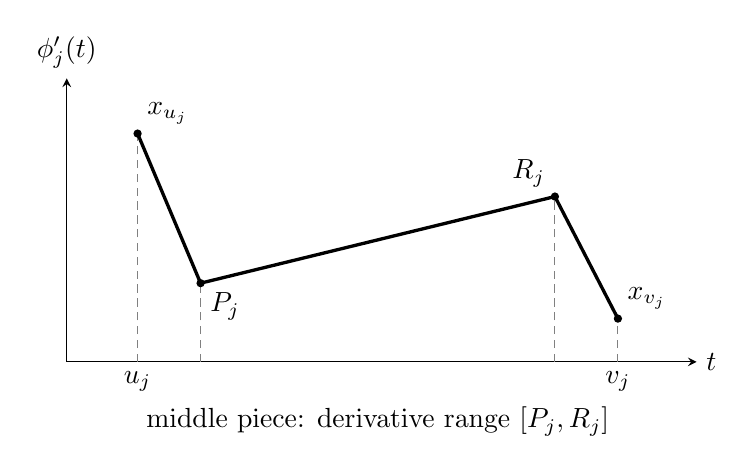
\begin{tikzpicture}[x=1cm,y=1cm,>=stealth]
 \draw[->] (0,0) -- (8,0) node[right] {$t$};
 \draw[->] (0,0) -- (0,3.6) node[above] {$\phi_j'(t)$};
 \draw[densely dashed,gray] (.9,0) -- (.9,2.9);
 \draw[densely dashed,gray] (1.7,0) -- (1.7,1.0);
 \draw[densely dashed,gray] (6.2,0) -- (6.2,2.1);
 \draw[densely dashed,gray] (7.0,0) -- (7.0,.55);
 \draw[very thick] (.9,2.9) -- (1.7,1.0) -- (6.2,2.1) -- (7.0,.55);
 \fill (.9,2.9) circle (1.5pt) node[above right] {$x_{u_j}$};
 \fill (1.7,1.0) circle (1.5pt) node[below right] {$P_j$};
 \fill (6.2,2.1) circle (1.5pt) node[above left] {$R_j$};
 \fill (7.0,.55) circle (1.5pt) node[above right] {$x_{v_j}$};
 \node[below] at (.9,0) {$u_j$};
 \node[below] at (7.0,0) {$v_j$};
 \node[below,align=center] at (3.95,-.45) {middle piece: derivative range $[P_j,R_j]$};
\end{tikzpicture}
\caption{A schematic leading phase derivative on one gap.  The short
outer pieces join the prescribed endpoint values to $P_j$ and $R_j$.
Their slopes may have either sign; the middle slope is positive.
The drawing shows one possible ordering of the endpoint values, and is
not to scale.}\label{fig:gap-derivative}
\end{figure}

Let $m_j$ interpolate linearly between the endpoint moduli $m_a$, with
modulus $1$ prescribed at $0$ and $1/2$.  Define on gap $j$
\begin{equation}\label{eq:gap-wave}
 B_N(t)=m_j(t)\e\bigl(N\phi_j(t)+\gamma_{j,N}(t)\bigr),
\end{equation}
where $\gamma_{j,N}$ is affine.  Choose its two endpoint values in
$[0,1)$ to give the exact phase factors required by the adjoining main
waves, and phase factor $1$ at $0$ and $1/2$.  There is no constraint on
these choices: each endpoint requires just one congruence modulo $1$.
In particular,
\[
 \int_{u_j}^{v_j}|\gamma_{j,N}'(t)|\,dt\le1,
 \qquad |\gamma_{j,N}'|\le l_j^{-1}.
\]
The second bound depends on the fixed gap but is independent of $N$.
Extend to the negative half-circle by
$B_N(-t)=\overline{B_N(t)}$.  Because $B_N(0)=B_N(1/2)=1$, this gives a
continuous function on $\T$ satisfying \eqref{eq:wave-modulus}.
On reflected gaps use the leading phase $-\phi_j(-t)$.  Its derivative is
$\phi_j'(-t)$, so the leading phase derivatives match across every join,
including $0$ and the identified endpoints $\pm1/2$.  Matching the full
derivatives of $B_N$ is unnecessary.

\subsection*{Fourier cost of the gaps}

We now bound the Fourier contributions of the gaps.  In
\eqref{eq:gap-wave} regard $f_N=m_j\e(\gamma_{j,N})$ as the amplitude.
On each piece,
\begin{equation}\label{eq:gap-amplitude-variation}
 \sup|f_N|+\int|f_N'|\le C
\end{equation}
with an absolute constant, since $m_j$ is monotone between values in
$[1,2]$ and the total variation of $\gamma_{j,N}$ is at most $1$.
Lemma~\ref{lem:oscillatory-bounds} and
\eqref{eq:gap-outer-slopes} show that all outer pieces and their
reflections contribute at most $C\sqrt\delta$ to the scaled Fourier
coefficient $\sqrt N\,\widehat B_N(k)$.

Choose a fixed $\rho>0$ so that the closed $\rho$-neighborhoods of the
finitely many derivative intervals $[P_j,R_j]$ are pairwise disjoint.
At most one of these intervals is within $\rho$ of $x=k/N$.  If such an
interval exists, the quadratic estimate and \eqref{eq:gap-middle-slope}
bound the total contribution of its middle piece and its reflection by
$C\sqrt L$.
Every other middle piece has monotone $\phi_j'-x$ of modulus at least
$\rho$.  The first-derivative estimate in
Lemma~\ref{lem:oscillatory-bounds}, together with
\eqref{eq:gap-amplitude-variation}, bounds its scaled contribution by
$C/(\rho\sqrt N)$.  The same bound holds for its reflection.  Their
number and $\rho$ are fixed, so the sum of these terms is $o(1)$,
uniformly in $k$.  Combining these bounds with
\eqref{eq:main-fourier-bound} proves
\[
 \sqrt N\,|\widehat B_N(k)|
 \le1+2\delta+C\sqrt\delta+C\sqrt L+o(1)
 \le1+C\sqrt\delta+o(1),\qquad 0\le k<N.
\]
Increasing $N_0(\delta)$ absorbs the last error into $\sqrt\delta$ and
proves \eqref{eq:wave-coefficients}.  In particular, neither the number
of gaps nor their separation contributes to the surviving constant.

\subsection*{Cancellation at the joins and the exterior tail}

For projection to the allowed frequencies, an estimate on individual
exterior coefficients is insufficient; we need their sum to tend to
zero.  This is where matching the leading phase derivatives is used.
Partition $[-1/2,1/2]$ into all main intervals and the three pieces of each
gap and reflected gap.  On each piece write
\[
 B_N(t)=f_N(t)\e(N\phi(t)).
\]
The functions $f_N,f_N',f_N''$ are bounded independently of $N$ on each
piece.  The phase $\phi$ is fixed, its first three derivatives are
bounded, and all values of $\phi'$ lie in a fixed compact subinterval of
$(0,1)$.  These bounds may depend on all the fixed construction data.
For $k<0$ or $k\ge N$, put $D=N+|k|$ and $V=N\phi'-k$.  Then
\begin{equation}\label{eq:exterior-phase-bounds}
 |V|\ge cD,\qquad |V'|+|V''|\le C_*N
\end{equation}
on every piece, for fixed $c>0$ and $C_*<\infty$.

The first integration by parts gives boundary terms
\[
 \frac{f_N(t)\e(N\phi(t)-kt)}{2\pi iV(t)}
 =\frac{B_N(t)\e(-kt)}{2\pi i(N\phi'(t)-k)}.
\]
They cancel at every internal join, because $B_N$ is continuous and the
leading phase derivatives agree.  They also cancel at $-1/2$ and $1/2$:
there $B_N=1$, $\phi'=1/8$, and
$\e(-k/2)=\e(k/2)$ for integer $k$.
After this cancellation, a second integration by parts involves
\[
 A:=\frac{(f_N/V)'}{V}
 =\frac{f_N'}{V^2}-\frac{f_NV'}{V^3}
\]
and its derivative
\[
 A'=\frac{f_N''}{V^2}
 -\frac{3f_N'V'}{V^3}
 -\frac{f_NV''}{V^3}
 +\frac{3f_N(V')^2}{V^4}.
\]
Since $N\le D$, \eqref{eq:exterior-phase-bounds} implies
$|A|+|A'|\le C_{\mathrm{data}}D^{-2}$.  Both the second boundary terms
and the remaining integrals therefore have this bound on each piece.
There are only finitely many pieces, whence
\[
 |\widehat B_N(k)|\le C_{\mathrm{data}}(N+|k|)^{-2}
 \qquad(k<0\text{ or }k\ge N).
\]
Summing over these integers proves \eqref{eq:wave-tail}, since
$\sum_{k\in\Z}(N+|k|)^{-2}=O(N^{-1})$.
The finitely many interior coefficients and this summable exterior bound
show that the full Fourier series converges absolutely.  Its sum equals
$B_N$ by continuity and uniqueness of Fourier coefficients.  Finally,
conjugate symmetry gives $\widehat B_N(k)\in\R$ for every integer $k$.
\end{proof}

\section{Projection and rounding to real signs}\label{sec:completion}

We now complete the proof of Theorem~\ref{thm:main}. The functions in
Proposition~\ref{prop:waves} already have almost constant modulus.
Their Fourier coefficients are real and lie in an almost unit cube
after multiplication by $\sqrt N$. Their large $L^2$ norm forces
most of these coefficients to be close to signs, exactly the condition
needed by Lemma~\ref{lem:complex-rounding}.

Fix a sufficiently small $\delta>0$, and let $B_N$ be supplied by
Proposition~\ref{prop:waves}. Choose an absolute constant $C_1$ so that
\[
 S_\delta=1+C_1\sqrt\delta,
 \qquad Y_k=\frac{\sqrt N}{S_\delta}\widehat B_N(k)
 \quad(0\le k<N)
\]
satisfy $Y_k\in[-1,1]$ for every sufficiently large $N$.
The symmetry $B_N(-t)=\overline{B_N(t)}$ makes every Fourier
coefficient real. Set
\[
 U_Y(t)=\frac1{\sqrt N}\sum_{k=0}^{N-1}Y_k\e(kt).
\]
The absolute Fourier representation and exterior-tail estimate in
Proposition~\ref{prop:waves} give
\begin{equation}\label{eq:projection-uniform}
 U_Y=B_N/S_\delta+O_\delta(N^{-1})
 \quad\text{uniformly on }\T.
\end{equation}
Parseval's identity and $|B_N|\ge1$ consequently imply
\[
 \frac1N\sum_{k=0}^{N-1}Y_k^2\ge S_\delta^{-2}-o(1).
\]
Here and below $N\to\infty$ with all the data chosen from $\delta$
fixed. Since $|Y_k|\ge Y_k^2$, the defect satisfies
\[
 \frac\mu N:=\frac1{2N}\sum_{k=0}^{N-1}(1-|Y_k|)
 \le\tfrac12(1-S_\delta^{-2})+o(1).
\]
Put $q_\delta=\tfrac12(1-S_\delta^{-2})+\delta$.
Then $q_\delta\to0$ as $\delta\downarrow0$, and for all sufficiently
large $N$ we have $\mu/N\le q_\delta<1/2$.

Lemma~\ref{lem:complex-rounding}, applied to these real inputs, produces
$\varepsilon_k\in\{-1,1\}$ such that
\[
 U_\varepsilon(t)=\frac1{\sqrt N}\sum_{k=0}^{N-1}\varepsilon_k\e(kt)
 \quad\text{satisfies}\quad
 \norm{U_\varepsilon-U_Y}_\infty
 \le C\left(N^{-1/2}+
        \sqrt{q_\delta\log(80/q_\delta)}\right).
\]
We used the monotonicity of $q\log(80/q)$ on $(0,1/2]$;
the zero-defect case causes no change. If
$E_\delta=C\sqrt{q_\delta\log(80/q_\delta)}$, the two-sided modulus
bound in Proposition~\ref{prop:waves} and
\eqref{eq:projection-uniform} give, uniformly in $t$,
\[
 S_\delta^{-1}-E_\delta-o(1)
 \le |U_\varepsilon(t)|
 \le \frac{1+C\delta}{S_\delta}+E_\delta+o(1).
\]
For fixed $\delta$, the $o(1)$ terms vanish as $N\to\infty$;
the resulting bounds both tend to $1$ as $\delta\downarrow0$.
Given the $\varepsilon$ of Theorem~\ref{thm:main},
choose $\delta$ so that the limiting bounds lie strictly between
$1-\varepsilon$ and $1+\varepsilon$, and then take $N$ large enough
to absorb the displayed errors. This proves the theorem.

The construction imposes no divisibility condition on $N$.
All torus dimensions, packing parameters, intervals, and leading phases were
fixed before $N$ was chosen. The phase identities use only that the
Fourier index $k$ is an integer. The conclusion therefore holds for
every sufficiently large integer length.

\bibliographystyle{plain}
\bibliography{references}
\end{document}
